\begin{figure*}
\centering
\begin{subfigure}[b]{0.48\textwidth}
    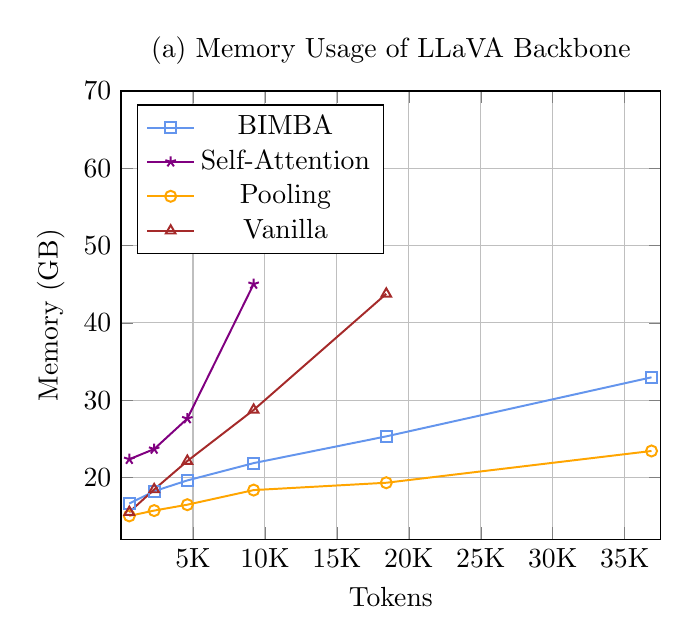
\begin{tikzpicture}
    \begin{axis}[
        % width=12cm, height=8cm,
        xlabel={Tokens},
        ylabel={Memory (GB)},
        title={(a) Memory Usage of LLaVA Backbone},
        xmin=0, xmax=37500,
        ymin=12, ymax=70,
        %xtick={576, 2304, 4608, 9216, 18432, 36864},
        % xticklabels={576, 2304, 4608, 9216, 18432, 36864},
        xtick={5000, 10000, 15000, 20000,25000,30000, 35000},
        xticklabels={5K, 10K, 15K, 20K, 25K,30K, 35K},
        %ytick={62, 64, 66, 68, 70, 72, 74},
        legend pos=north west,
        grid=both,
        scaled ticks = false,
        scaled x ticks = false,
        % xmode=log,
        % log basis x=1
    ]
    % BIMBA Data
    \addplot[line width=.25mm, color=CornflowerBlue, mark=square, mark size=2pt]
    coordinates {
    (576, 16.62) (2304, 18.22) (4608, 19.61) (9216, 21.85) (18432, 25.31) (36864, 32.95)
    };
    \addlegendentry{BIMBA}
    
    % Self-Attention Data
    \addplot[line width=.25mm, color=Purple, mark=star, mark size=2pt]
        coordinates {
        (576, 22.35) (2304, 23.67) (4608, 27.61) (9216, 45.01)
    };
    \addlegendentry{Self-Attention}
    
    % Pooling Data
    \addplot[line width=.25mm, color=Orange, mark=o, mark size=2pt]
    coordinates {
    (576, 15.02) (2304, 15.71) (4608, 16.47) (9216, 18.36) (18432, 19.31) (36864, 23.42)
    };
    \addlegendentry{Pooling}

    %Vanilla
    \addplot[line width=.25mm, color=Brown, mark=triangle, mark size=2pt]
    coordinates {
    (576, 15.51) (2304, 18.44) (4608, 22.12) (9216, 28.73) (18432, 43.75)
    };
    \addlegendentry{Vanilla}

    \end{axis}
    \end{tikzpicture}
% \caption{Figure 1}
\end{subfigure}
\hfill
\begin{subfigure}[b]{0.48\textwidth}
    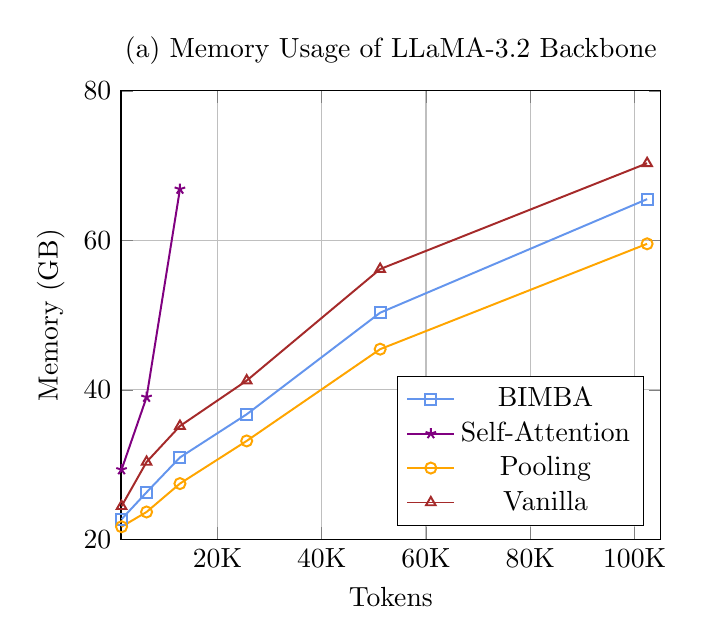
\begin{tikzpicture}
    \begin{axis}[
        % width=12cm, height=8cm,
        xlabel={Tokens},
        ylabel={Memory (GB)},
        title={(a) Memory Usage of LLaMA-3.2 Backbone},
        xmin=1500, xmax=105000,
        ymin=20, ymax=80,
        %xtick={1600, 6400, 12800, 25600, 51200, 102400},
        % xticklabels={1600, 6400, 12800, 25600, 51200, 102400},
        xtick={20000,40000,60000,80000,100000},
        xticklabels={20K, 40K, 60K, 80K, 100K},
        % ytick={67, 69, 71, 73, 75, 77},
        legend pos=south east,
        grid=both,
        scaled ticks = false,
        scaled x ticks = false,
        % xmode=log,
        % log basis x=1
    ]
    % BIMBA Data
    \addplot[line width=.25mm, color=CornflowerBlue, mark=square, mark size=2pt]
    coordinates {
    (1600, 22.68) (6400, 26.28) (12800, 30.95) (25600, 36.72) (51200, 50.32) (102400, 65.52)
    };
    \addlegendentry{BIMBA}
    
    % Self-Attention Data
    \addplot[line width=.25mm, color=Purple, mark=star, mark size=2pt]
        coordinates {
        (1600, 29.31) (6400, 39.01) (12800, 66.86) 
    };
    \addlegendentry{Self-Attention}
    
    % Pooling Data
    \addplot[line width=.25mm, color=Orange, mark=o, mark size=2pt]
    coordinates {
    (1600, 21.67) (6400, 23.65) (12800, 27.45) (25600, 33.16) (51200, 45.44) (102400,59.54)
    };
    \addlegendentry{Pooling}
    \addplot[line width=.25mm, color=Brown, mark=triangle, mark size=2pt]
    coordinates {
    (1600, 24.42) (6400, 30.34) (12800, 35.15) (25600, 41.23) (51200, 56.16) (102400, 70.32)
    };
    \addlegendentry{Vanilla}

    \end{axis}
    \end{tikzpicture}
    % \caption{Figure 2}
\end{subfigure}
\caption{Computation Costs of LLaVA Backbone}
\label{fig:memory}
\end{figure*}